%!TEX root = ../paper.tex


\section{Impact of Device Performance} \label{intro}

\begin{figure*}[t]
    \begin{subfigure}[b]{0.33\textwidth}
        \centering
        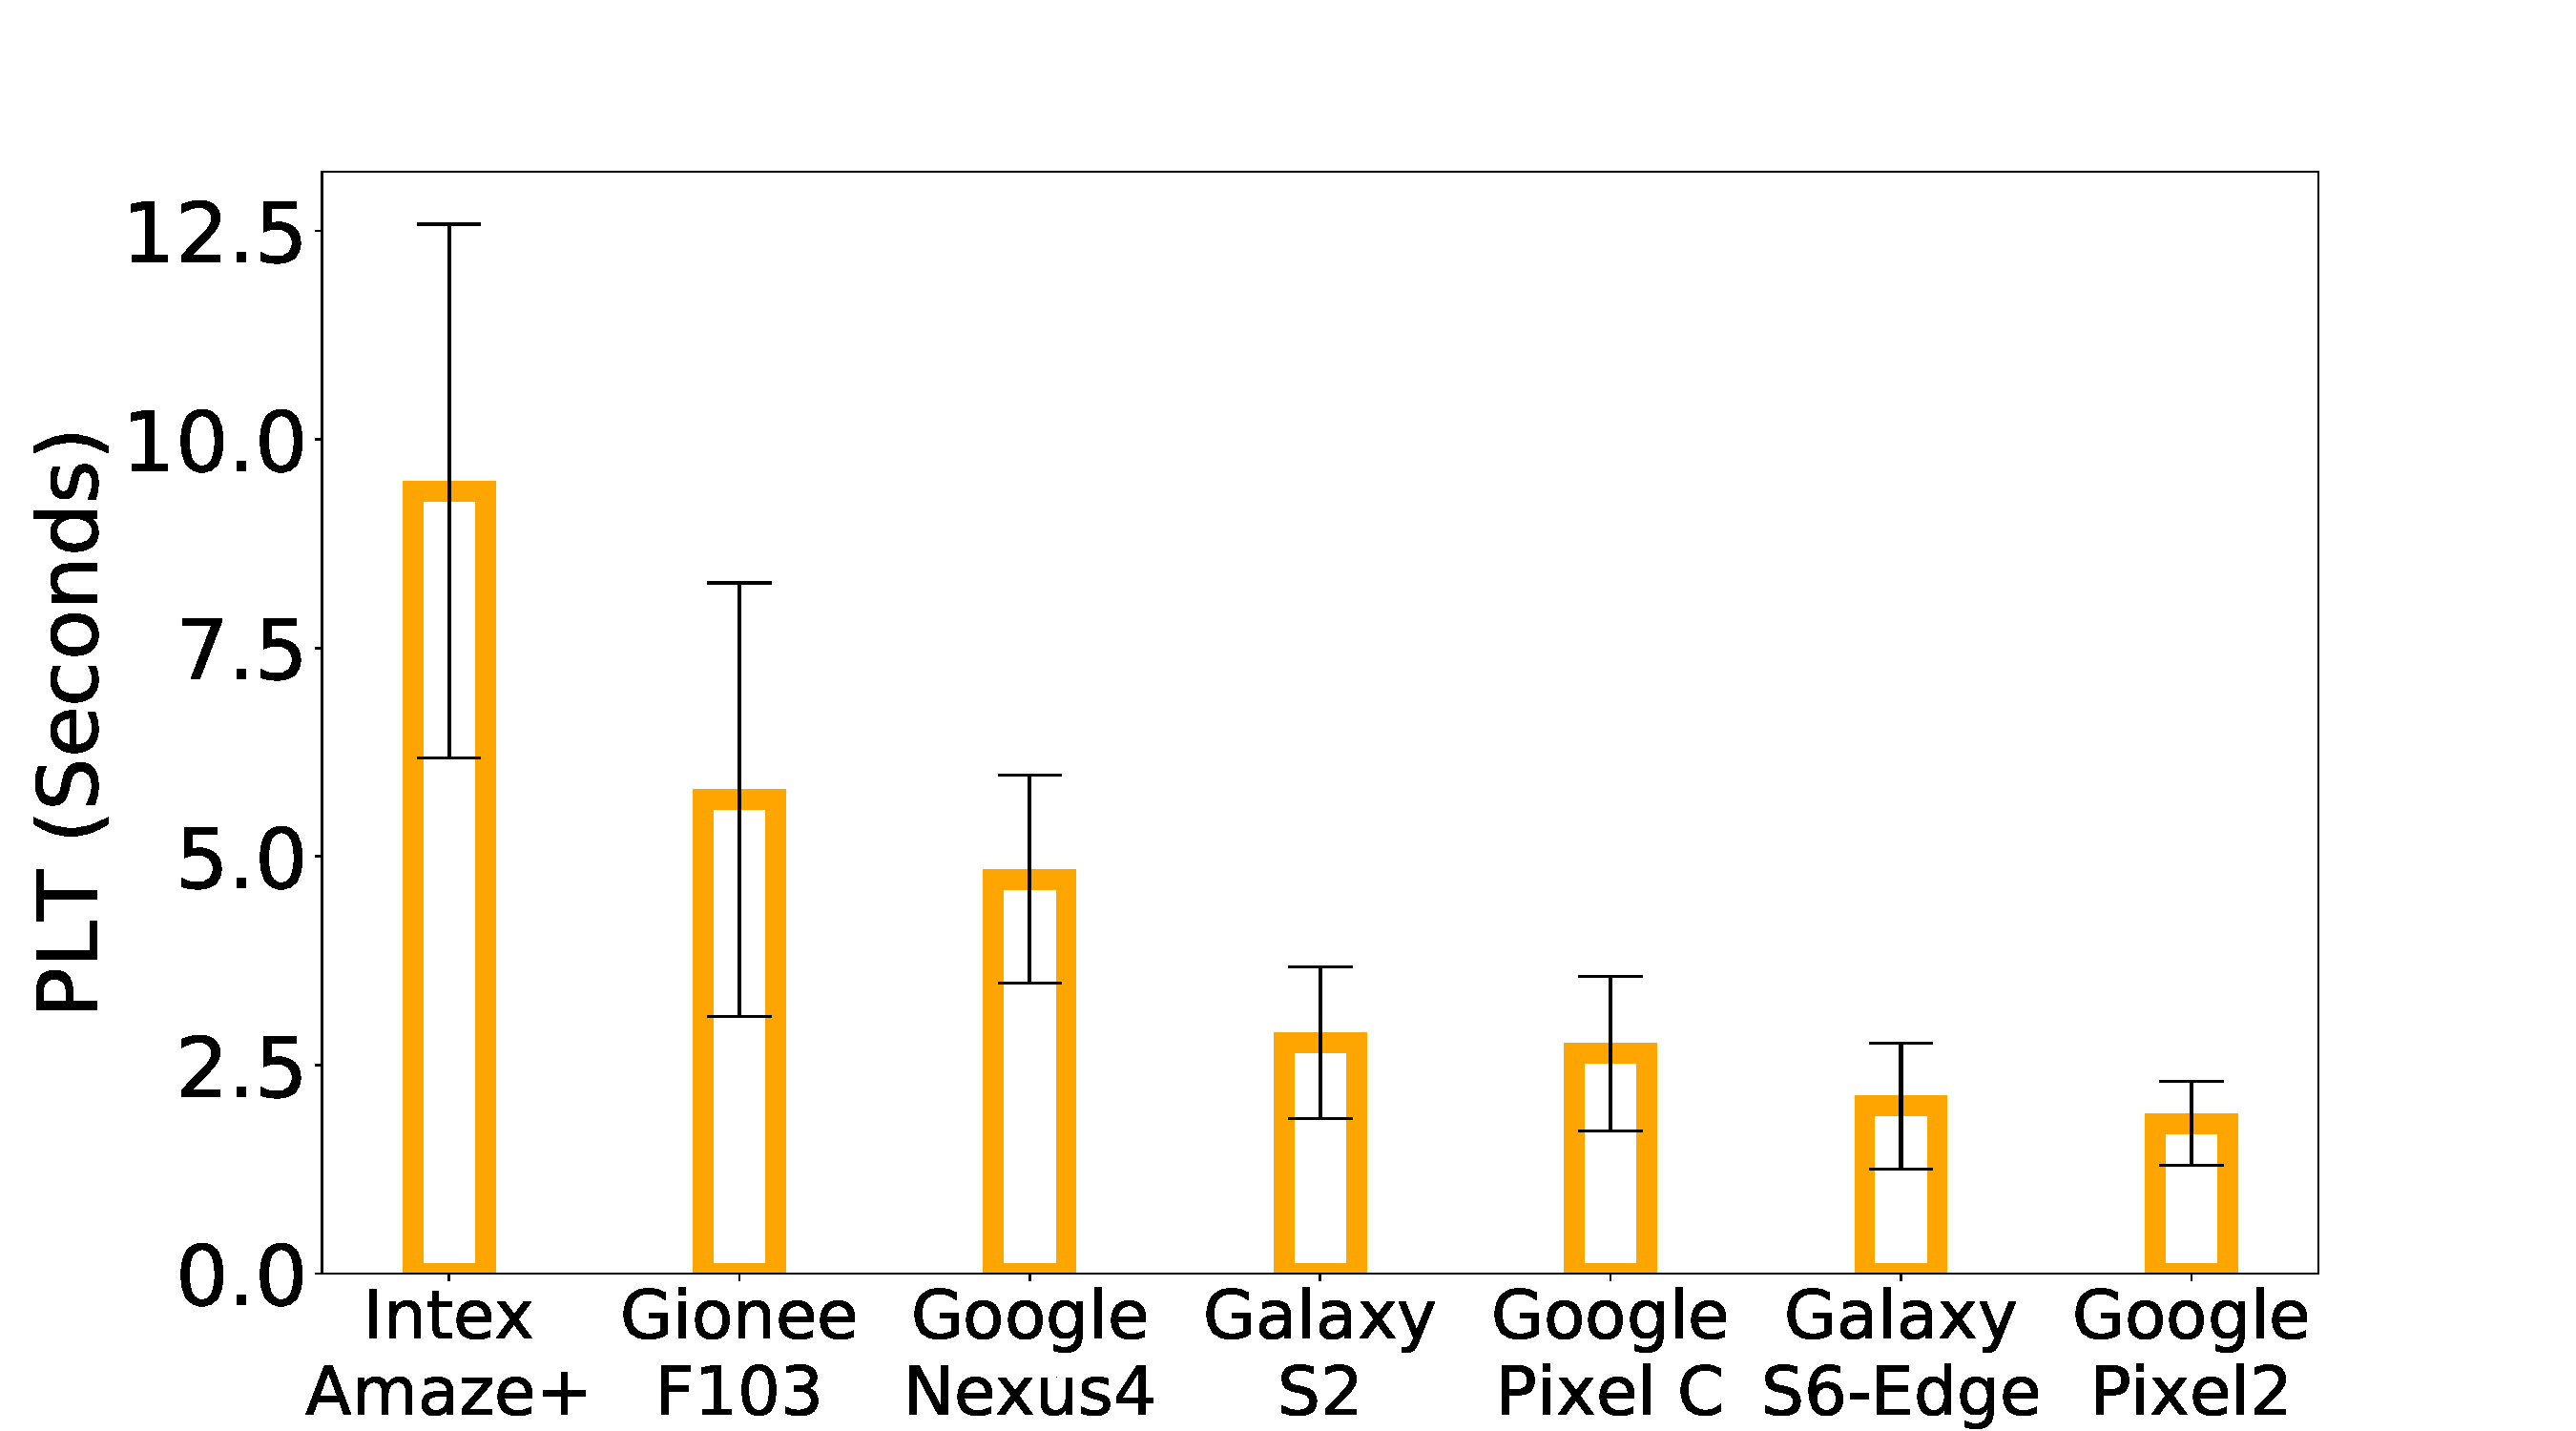
\includegraphics[width=1\linewidth]{sections/device-work/plt-devices}
        \caption{Web Browsing}
    \end{subfigure}
    \begin{subfigure}[b]{0.33\textwidth}
        \centering
        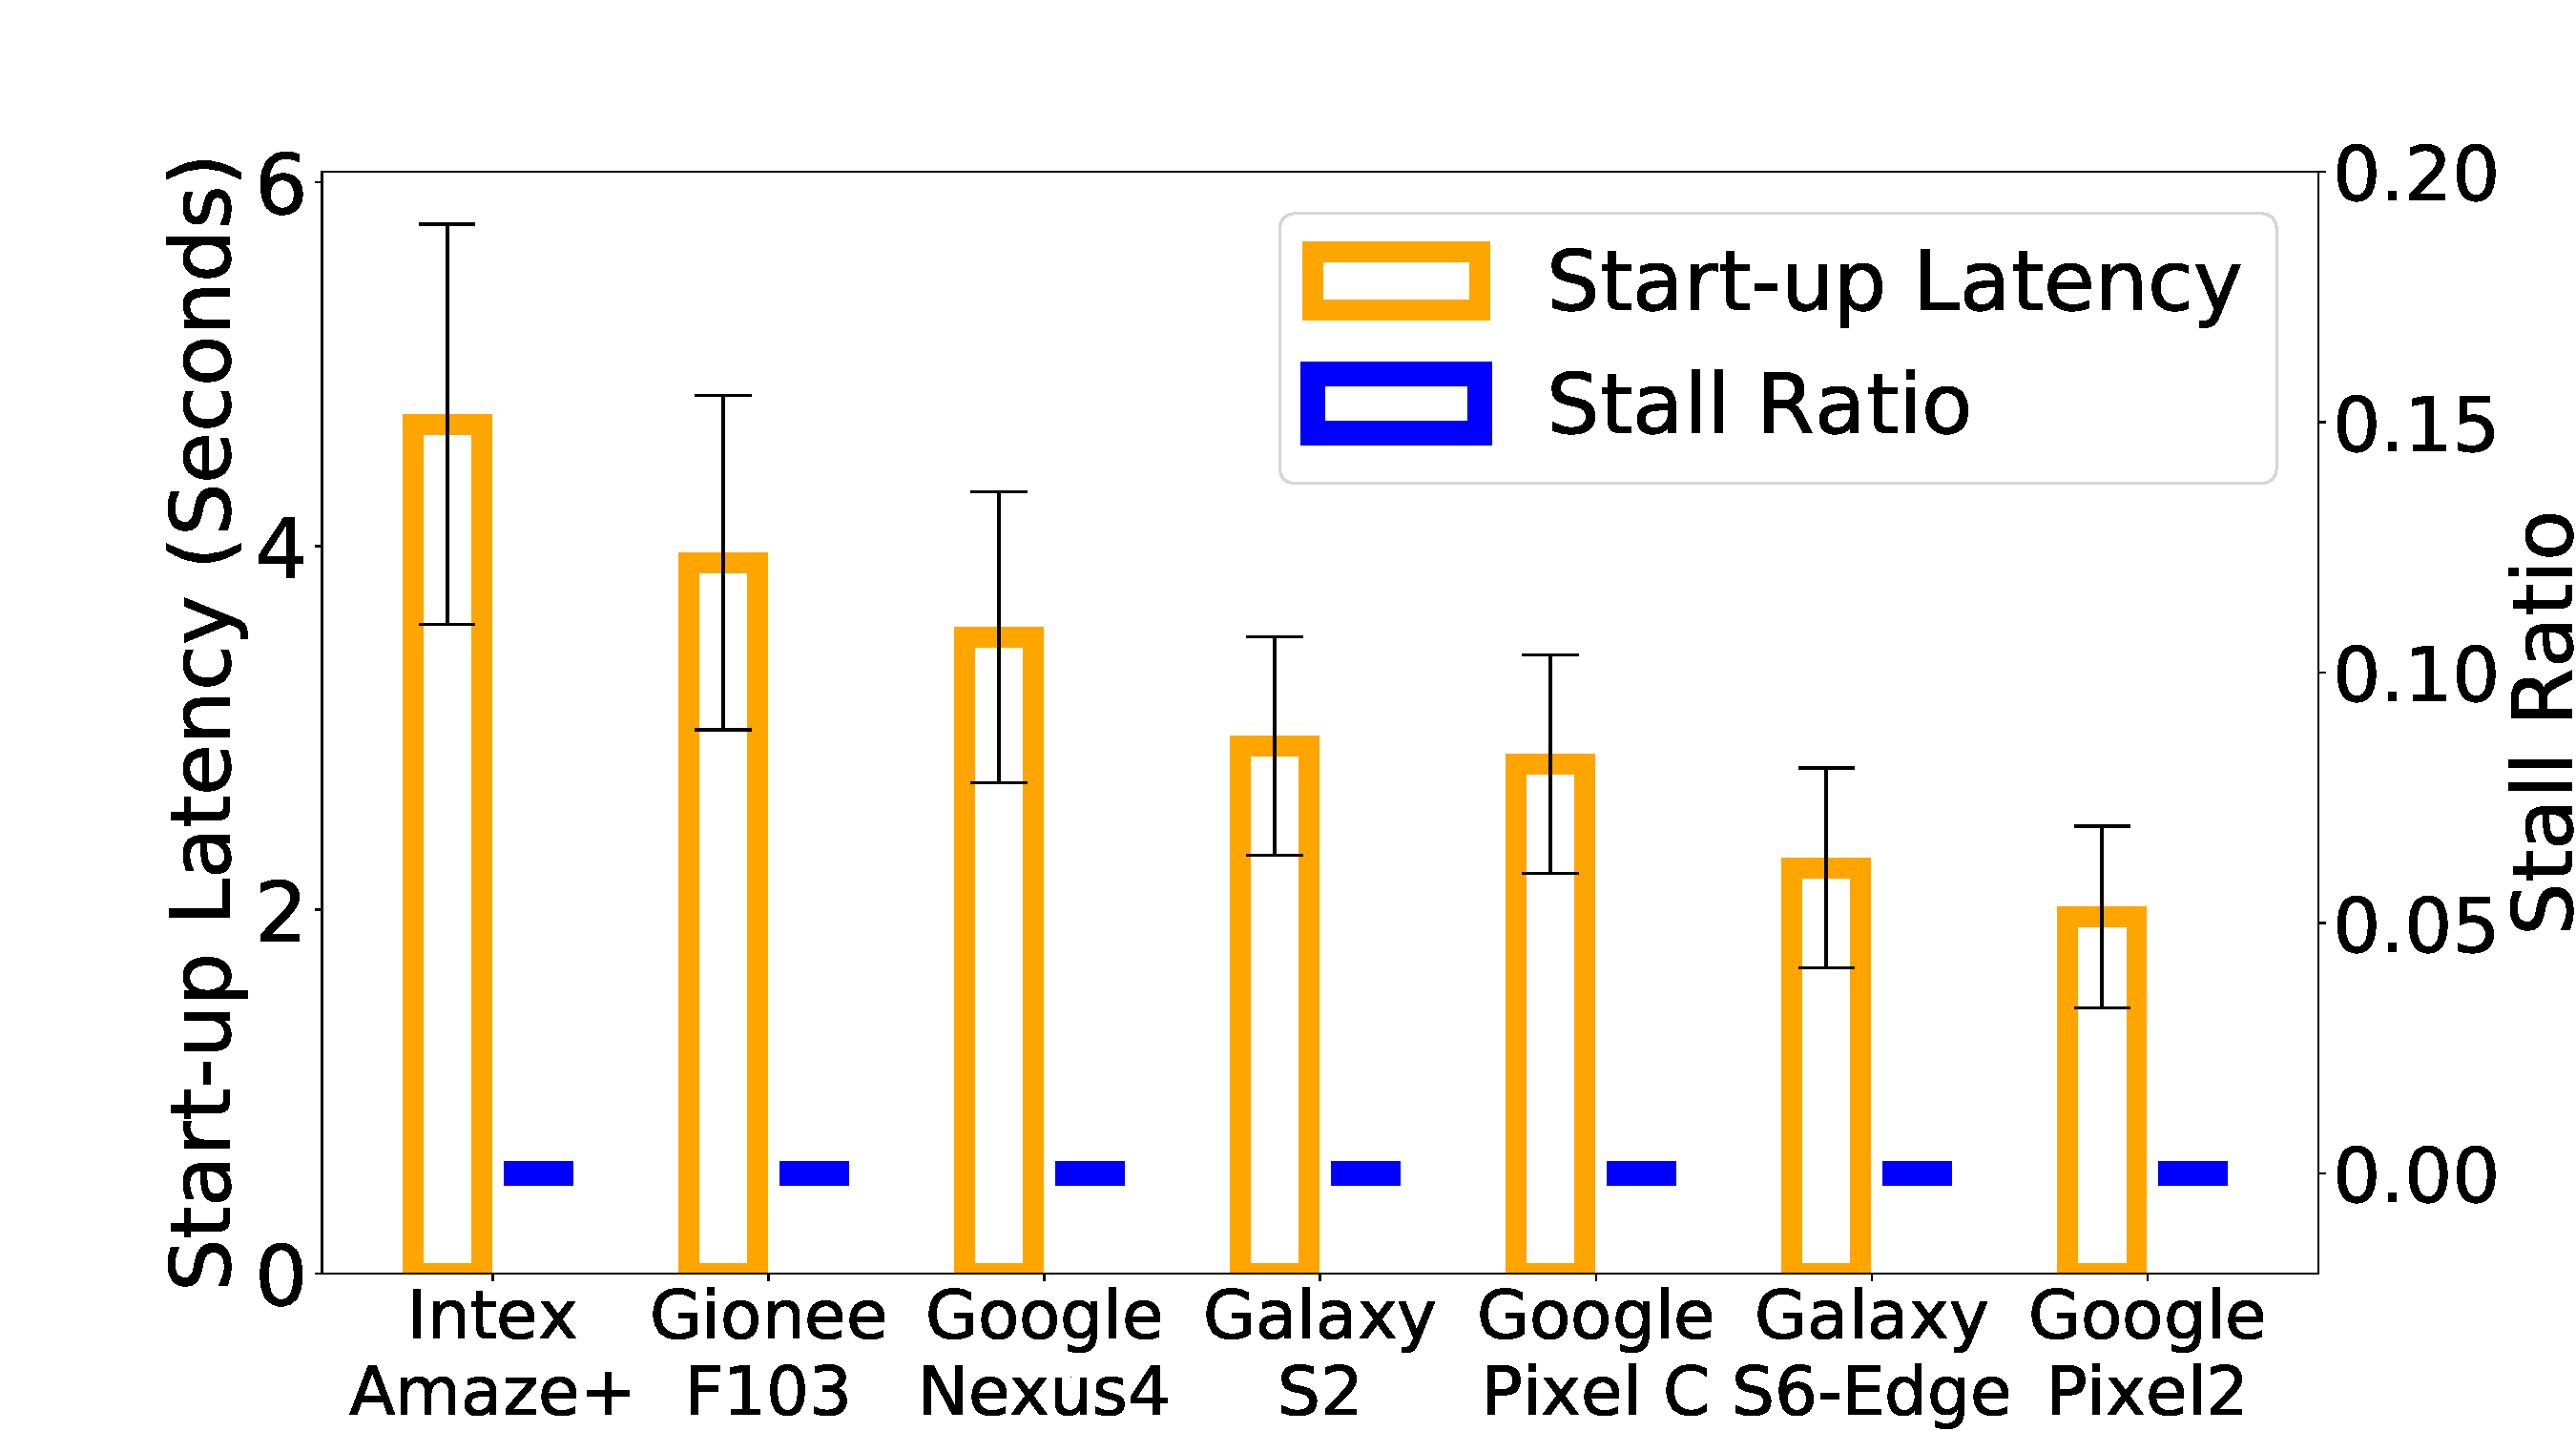
\includegraphics[width=1\linewidth]{sections/device-work/youtube-motivation}
        \caption{Video Streaming}
    \end{subfigure}%
    \begin{subfigure}[b]{0.33\textwidth}
        \centering
        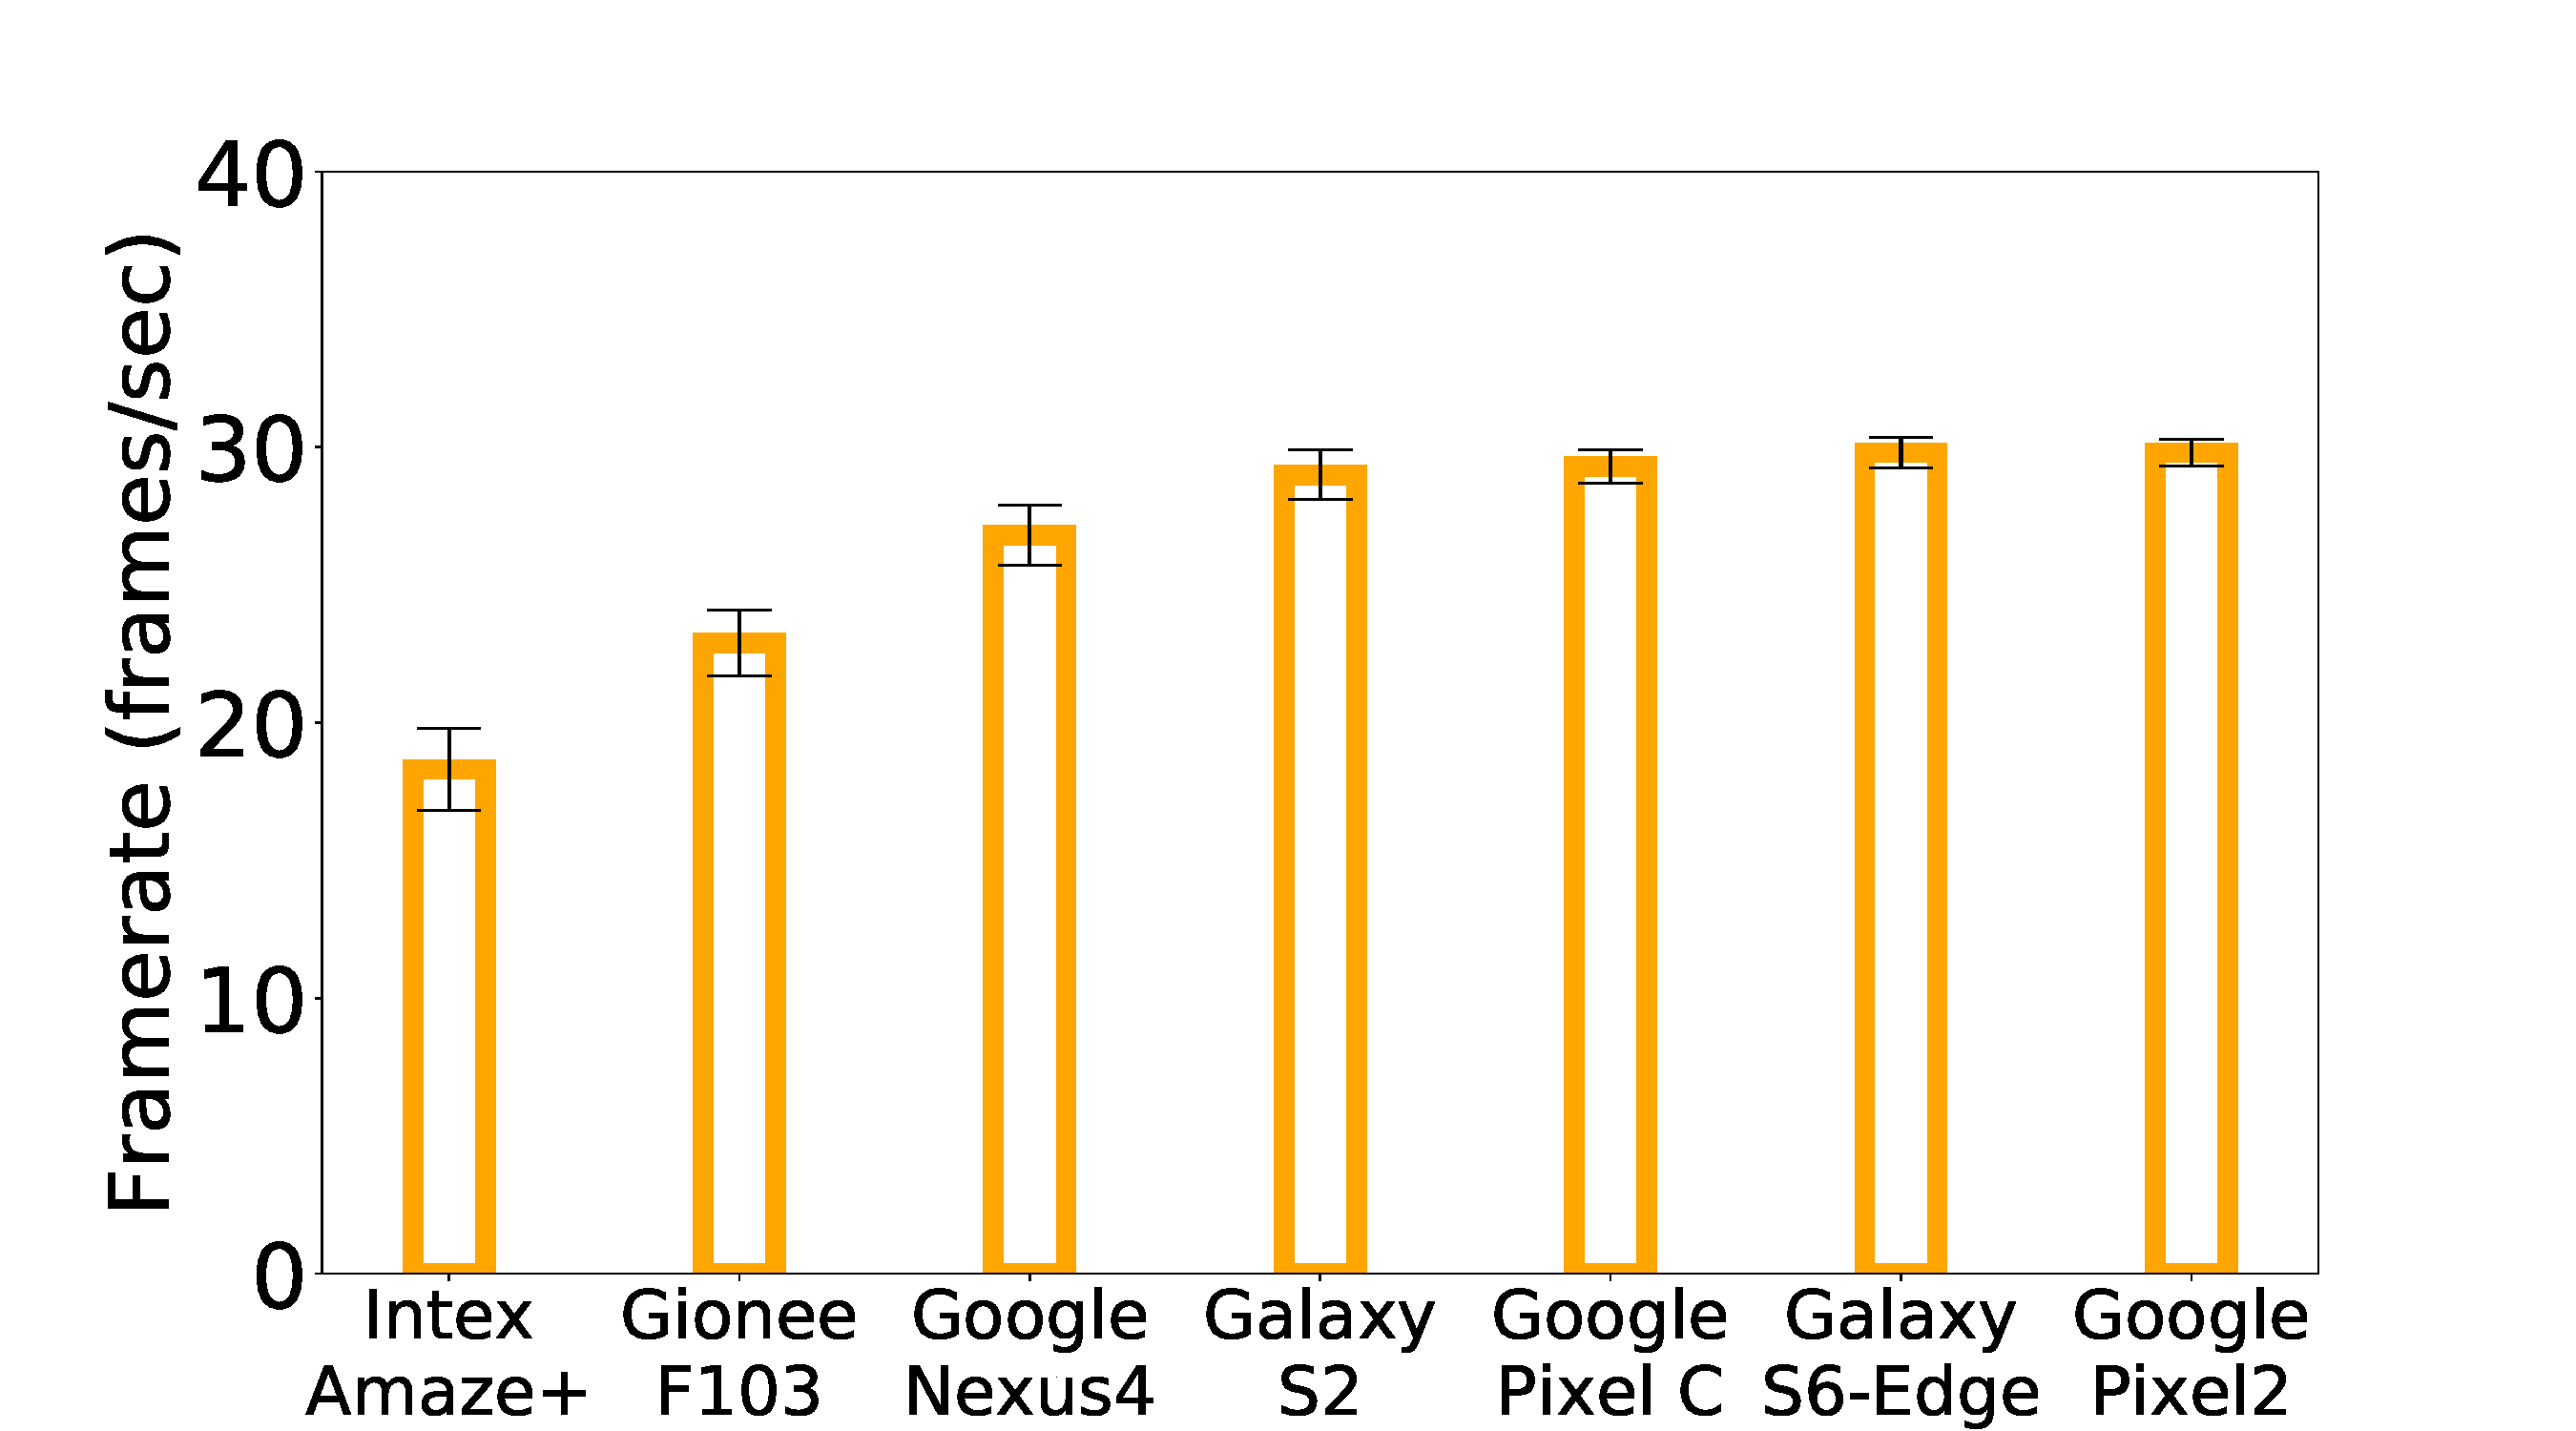
\includegraphics[width=1\linewidth]{sections/device-work/skype-motivation}
        \caption{Video Telephony}
    \end{subfigure}
     \caption{Mobile application performance across diverse devices: (a) Web Browsing, (b)Video Streaming, (c) Video Telephony. The horizontal axis shows the device type; their corresponding specifications are tabulated in Table~\ref{tab:device_types}.}
     \label{fig:motivation}
\end{figure*}

\begin{table*}[t]
  \centering
   \scalebox{0.9}{
  \begin{tabular}{c|c|c|c|c|c|c|c}
  \hline \hline
    \textbf{Device} & \textbf{Application} & \textbf{Number} & \textbf{OS} & \textbf{Clock} & \textbf{GPU} & \textbf{RAM} & \textbf{Release} \\
      \textbf{Name} & \textbf{Processor} & \textbf{of Cores} & \textbf{Version} & \textbf{Min-Max (Mhz)}  & \textbf{Type} & \textbf{Size (GB)} & \textbf{Cost} \\
    \hline
    \hline
    Intex Amaze+ &Spreadtrum SC9832A&4&6.0&300-1300 &Mali-400&1&\$60\\
    Gionee F103 &MediaTek MT6735&4&5.0&300-1300 &Mali-T720&2&\$150\\
    Nexus4 &Snapdragon S4 Pro&4&5.1.1&384-1512 &Adreno 320&2&\$200\\
    SG S2-Tab &Exynos 5433&8&5.0.2&400-1300 &Mali-T760&3&\$450\\ 
    Pixel-Tab &Tegra X1&4&8.0.0&204-1912& Maxwell&3&\$600\\ 
    SG S6-edge &Exynos 7420&8&6.0.1&400-2100 &Mali-T760&3&\$880\\
    Pixel2 &Snapdragon 835&8&8.0.0&300-2457 &Adreno 540&4&\$700\\ \hline \hline
  \end{tabular}
    }
  \caption{The table shows the set of diverse mobile devices used in our motivation experiment and their corresponding specifications including cost, CPU capabilities, and memory capacity. }%Mobile Devices in our Experiments showing OS/Hardware Specifications: Shown are parameters that impact the performance of mobile applications}
  \label{tab:device_types}
\end{table*}
While mobile smartphones have now penetrated 
a significant fraction of world population, the devices 
vary widely in terms of cost and performance. 
For example, the smartphones in the market 
range from $\approx$\$50 to $\approx$\$1000~\cite{mobilephones, contreras2017patents}, and the cost 
largely depends on the hardware specifications. 
For example, a \$600 phone such as OnePlus5 has 8 cores, running upto 2.4\,Ghz clock and 6\,GB RAM, while a cheaper \$60 phone (e.g., Dell Venue Pro) only has 2 cores with up to 1\,GHz clock and 512\,MB RAM. 

However, the impact of the hardware specs
on the performance of mobile Internet applications is not well-studied. A large fraction of past research on mobile Internet performance has focused on the effect of the {\em network} on the applications~\cite{butkiewicz2015klotski, kelton2017improving, singh2015flexiweb, Ruamviboonsuk:2017:VAM:3098822.3098851, Shafiqund, Xiaodash2m, chen2016effective} but not 
the device. Some studies do address the compute performance of mobile Internet applications~\cite{zhu2017optimizing,jones2009parallelizing,mai2012case}, but the underlying
technologies developed are more suited for higher end devices. 

Given that a large fraction of mobile
users in developing regions (62\%-68\% by some 
account \cite{unity}) uses smartphones with relatively
less expensive lower end hardware, it is important
to understand the impact of the device hardware on the 
performance of the mobile apps. In fact, with the increased 4G penetration, network speed is no longer the bottleneck in many developing countries~\cite{mobilephones,contreras2017patents,jioplans1,jioplans2}.  Our measurements show that mobile Web page loads on two popular phones in India, Intex Amaze 4 ($\approx$\$60) and Gionee ($\approx$\$150) are $5\times$ to $3\times$ worse, respectively, compared to Web page loads on Google Pixel2 ($\approx$\$700) under the same network conditions (\S\ref{sec:motivation}). 
This underscores the importance of studying the influence of the device hardware
on the performance and explore ways to improve the mobile web experience on lower end hardware. 

In this paper, we focus on three types of mobile Internet applications:  {\em (i)} Web browsing, {\em (ii)} video streaming, and {\em (iii)} video telephony. We study performance in terms of Quality of Experience (QoE) and energy. We especially focus on how the {\em CPU clock frequency} impacts performance 
given that the clock frequency
has the most impact on the performance
among other aspects of the specification (\S\ref{sec:impact_cpu}).% varies  important resource that changes across low-end and high-end devices as the representative   
%However, our experiments show that the CPU clock has the most impact on application performance among these resources (\S\ref{sec:impact_cpu}). 
%For example, \todo{write something here to convince that this is the case}.
%\mallesh{We show this by measuring Web performance under different clock, memory and GPU conditions on Nexus4 phone. We find a low memory of 512MB RAM has an impact of 4 seconds increase in PLT while a lower clock of 384Mhz shows 11 seconds increase in PLT. We also measure the impact of disabling GPU, which has a 0.5 seconds difference from normal PLT which is 3.5 seconds. This shows that Clock frequency has an exponential increase in PLT.}
%The second problem that we solve is curating different hardware conditions. It is difficult to measure the application performance on various smartphones available in the market. So we take the approach of emulating these diverse smartphones by using a representative hardware parameter of smartphones. In our research, we find clock frequency of CPU is a key factor in application performance. Clock frequency directly determines the amount time required for certain computation. Hence, we use clock frequency parameter to emulate different smartphones because we find smartphones with clock frequency ranging from 300Mhz to 2.4Ghz in the market. We change the clock frequency with the help of clock frequency scaling algorithm called governor (Userspace) provided by Andriod. This allows us to fix the CPU clock on a smartphone.
%The QoE of an Internet application depends on several factors apart from the device hardware, including the network condition, the server, and other factors in the data delivery path. The problem is these factors are interdependent on one another (for example, impact of hardware on network apart from application computation). 

One of our key findings is that a slow CPU speeds not only affects compute performance, but has a second-order effect on the network
performance. In our measurements, for example, the TCP performance drops more than 20\,Mbps, 
when the CPU clock of the phone drops from 1512\,Mhz to 384\,Mhz. This is owing to 
the fact that a slower clock
increases TCP processing delays by as much 
as $\approx$12\,ms.
%In our experiments, the time between when the packet reached the kernel to when it reached the application differs by as much as 11ms between a slow and a fast CPU. 
The implication is that the application is doubly 
impacted by the slower clock that slows
down both the network latency/throughput as well as the compute 
performance inside the application. 
%since Internet application performance depends on both the network and the compute performance. 
% to low clock frequencies---affecting both compute and network. Application performance is a combination of the network performance, involving loading network objects, and computation performance, involving processing. 

Our goal now is in {\em isolating} the effect of CPU clock on the network and the compute activities of the application. This isolation is critical to shed light on how the application 
performance can be improved for low-end devices: should the optimization focus on improving the TCP packet processing or the application compute? While straightforward for video applications, for Web browsing, this isolation is challenging.  
Loading of Web objects, a network process, and processing of these objects, a compute process, are intertwined during the page load process and cannot be cleanly separated. To this end, we leverage the WProf tool~\cite{wang2013demystifying,nejati2016depth} that breaks down the Web page load process into network and compute processes on the critical path. The key findings of our study are: %In the case of video applications, we isolate the effect of network and compute by

\begin{itemize}    

   \item {\bf Mobile Web performance is significantly affected by slow clocks:} Web page loads slow down by a
    factor of 5 on average when CPU clock speed reduces from 1512 Mhz to 384 Mhz. This slow down is both because of compute processing delays and the second-order effect in network processing. Our isolation experiments show that compute processing is more of a bottleneck under slow CPU speeds, accounting for over 60\% of the 
    page load time. Within the compute activities, Javascript evaluation is affected most by 
    the CPU slow down, and rendering and painting are affected the least.
 
 %  the web page load slowed down by an average of 6 times across XXX Web pages, even when the network condition is held a constant. Under slow CPU clock, the processing of the Web objects slowed down, but the network loading is also affected because of the second-order effect described earlier. Using our isolation technique, we find that compute accounts for XXX of the slow down under low clocks. This result suggests that improving Web performance for low-end phones should focus on improving the performance of compute. 
   
   %The Web page load process consists of both network activities for loading objects, and compute activities for parsing HTML, running scripts, and rendering. Reducing CPU speeds both affects the compute activities directly, and the network downloads through the second order effect described earlier. To isolate this, we build an emulator which schedules object downloads by keeping the compute the constant. While scheduling object downloads, we preserve the dependencies captured using WProf tool. 

    \item {\bf A slow clock does not significantly affect video streaming because of offloading and pre-fetching:} 
    The QoE of video streaming is largely unaffected by slow CPU speeds, despite video streaming being a compute-intensive application. By isolating the impact of compute and network, we find that this paradox is because of two reasons. From the compute standpoint, 
     streaming applications use special hardware decoders, even available on low-end phones, to process video data rather than decode on the CPU.   %(e.g, \texttt{OMX.sprd.h264.decoder}). 
    From the networking standpoint, streaming applications pre-fetch enough data and are unaffected by the second-order network slow-downs caused by slow CPU. 
    
 %\item {\bf  Increasing CPU speeds beyond a inflection point has poor performance/power trade-off:} For all three applications, increasing  CPU speeds significantly increases energy consumption. However, the corresponding improvement in performance beyond a point is not commensurate with the energy cost. 

 \item {\bf Leveraging hardware offloading is a promising approach to improve Web performance under slow clock:}  Similar to the hardware offloading techniques used in video applications, offloading Javascript to a low-power DSP can potentially improve Web performance. Our preliminary 
 analysis with offloading only regular expression evaluations
shows that the improvement can be as much as 18\% in page load time along with a $4\times$ 
improvement in power consumption. %\todo{check the numbers.} 
\end{itemize}


